%----------------------------------------------------------------------------
\appendix
%----------------------------------------------------------------------------
\chapter*{Függelék}
\setcounter{chapter}{6}  % a fofejezet-szamlalo az angol ABC 6. betuje (F) lesz
\setcounter{equation}{0} % a fofejezet-szamlalo az angol ABC 6. betuje (F) lesz
\numberwithin{equation}{section}
\numberwithin{figure}{section}
\numberwithin{lstlisting}{section}
\numberwithin{table}{section}
\setcounter{footnote}{0}

%,,,,,,,,,,,,,,,,,,,,,,,,,,,,,,,,,,,,,,,,,,,,,,,,,,,,,,,,,,,,,,,,,,,,,,,,,,,,
\section{Paraméterezés}\label{sect:parameterezes}
%,,,,,,,,,,,,,,,,,,,,,,,,,,,,,,,,,,,,,,,,,,,,,,,,,,,,,,,,,,,,,,,,,,,,,,,,,,,,

\subsection{Pupillakeresés}

\begin{itemize}
  \item \textbf{küszöbözés} -- küszöbérték: 5
  \item \textbf{kontúrméret} -- terület legalább 2500 egység
  \item \textbf{körkörösség} -- 1,07-nél kisebb érték (1,0 a tökéletes kör)
\end{itemize}

\subsection{Validációs mérések}

A validációs méréseket a következő elrendezésben hajtottam végre:

\begin{itemize}
  \item 1280$\times$1024 képpont felbontású monitor, 37,5$\times$30,5 cm fizikai mérettel
  \item 33 cm magas álltámasz, középpontja a monitor közepétől 48 cm-re
\end{itemize}

%,,,,,,,,,,,,,,,,,,,,,,,,,,,,,,,,,,,,,,,,,,,,,,,,,,,,,,,,,,,,,,,,,,,,,,,,,,,,
\section{Környezet}\label{sect:telepites}
%,,,,,,,,,,,,,,,,,,,,,,,,,,,,,,,,,,,,,,,,,,,,,,,,,,,,,,,,,,,,,,,,,,,,,,,,,,,,

A rendszer fejlesztése a következő szoftververziók felhasználásával történt egy \emph{Dell Inspiron R15} típusú \emph{Microsoft Windows 7} operációs rendszert futtató notebookon (2,53 GHz-es Intel Core i5 processzor, 4 GB rendszermemória).

Azonos, vagy kompatibilis verziók használatával a forráskód (lásd \sectref{mellekletek} függelék) bármely \emph{Qt} és \emph{OpenCV} által támogatott rendszerre fordítható.

Az \emph{OpenCV} könyvtárat a \emph{MinGW} csomagban található eszközökkel kell lefordítani\footnote{hivatalos leírás: \url{http://opencv.willowgarage.com/wiki/WindowsInstallGuide}}, a \emph{Qt} rendszerrel való kompatibilitás miatt.  

\begin{itemize}
  \item \textbf{OpenCV} -- 2.3.0
  \item \textbf{Qt} -- 4.7.4 (32 bit)
  \item \textbf{Qt Creator} -- 2.4.1 (rev. 8cd370e163)
\end{itemize}

\newpage
%,,,,,,,,,,,,,,,,,,,,,,,,,,,,,,,,,,,,,,,,,,,,,,,,,,,,,,,,,,,,,,,,,,,,,,,,,,,,
\section{Kibővített osztálydiagram}\label{sect:osztalydiagram}
%,,,,,,,,,,,,,,,,,,,,,,,,,,,,,,,,,,,,,,,,,,,,,,,,,,,,,,,,,,,,,,,,,,,,,,,,,,,,

\begin{figure}[!ht]
\centering
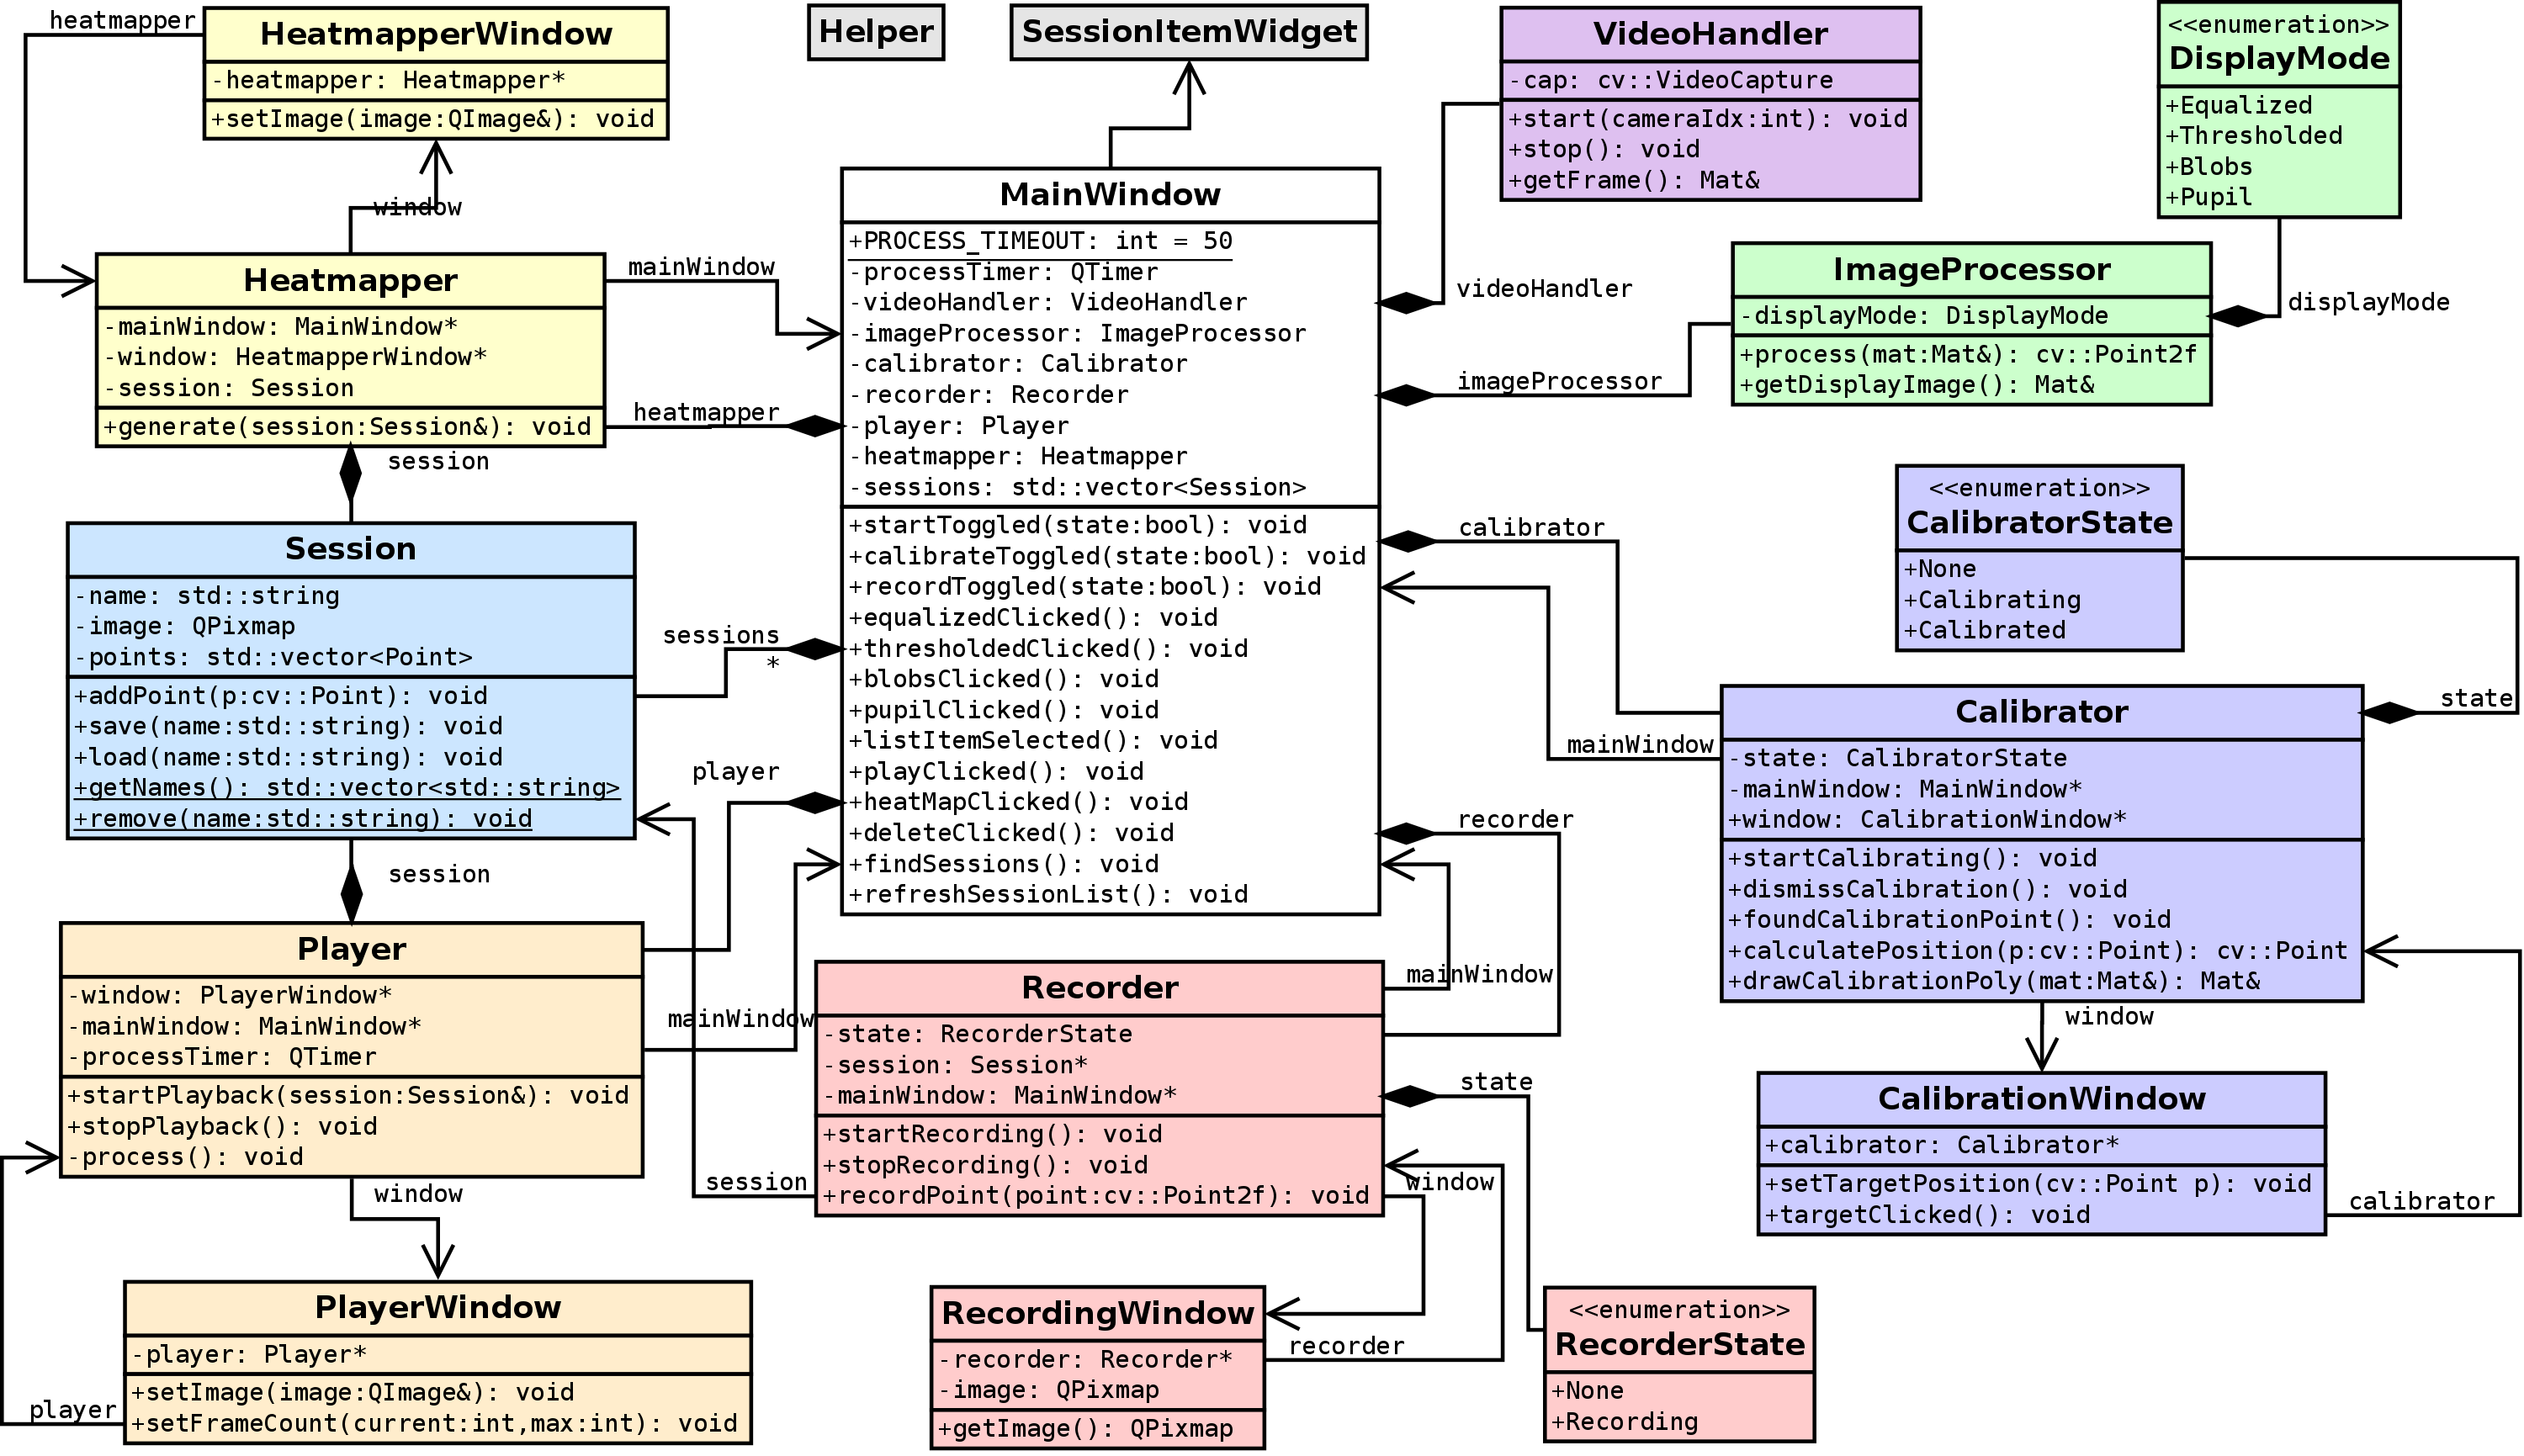
\includegraphics[width=130mm, keepaspectratio]{figures/class_diagram_aa.png}
\end{figure}


\newpage
%,,,,,,,,,,,,,,,,,,,,,,,,,,,,,,,,,,,,,,,,,,,,,,,,,,,,,,,,,,,,,,,,,,,,,,,,,,,,
\section{Mellékletek}\label{sect:mellekletek}
%,,,,,,,,,,,,,,,,,,,,,,,,,,,,,,,,,,,,,,,,,,,,,,,,,,,,,,,,,,,,,,,,,,,,,,,,,,,,

\subsection{Az Interneten}\label{sect:interneten}

A fejlesztés során elkészült alkalmazás forráskódja szabadon hozzáférhető egy \emph{GitHub}\footnote{közösségi kódbázis, lásd \url{http://www.github.com/}} projektben, a \textbf{\url{https://github.com/obrien/eyetracker}} címen.

A projekt nyitóoldala hivatkozásokat tartalmaz az elérhető mellékletekhez. 

\begin{itemize}
    \item \textbf{könyvtárak elérhetősége}
    \begin{itemize}
      \item az \textbf{OpenCV} könyvtár megfelelő verziója
      \item a \textbf{Qt} keretrendszer és a \textbf{Qt Creator} megfelelő verziója
    \end{itemize}
    
  \item \textbf{képgaléria}
    \begin{itemize}
      \item válogatás az alkalmazás tesztelése és használata során készített képekből
    \end{itemize}
    
  \item \textbf{videógaléria}
    \begin{itemize}
      \item pupillakövetési algoritmus működésének bemutatása
      \item videók a tekintetkövetés működéséről
    \end{itemize}

  \item \textbf{dokumentáció}
    \begin{itemize}
      \item a diplomatervem szövegének \LaTeX{} nyelvű forráskódja
      \item a diplomatervem PDF formátumban
    \end{itemize}
\end{itemize}

\subsection{CD-ROM-on}\label{sect:cdromon}

A fent felsorolt, online elérhető kiegészítéseket a diplomatervem CD-ROM mellékletén is elérhetővé tettem. A lemez könyvtárszerkezete és tartalma a következő.

\begin{itemize}
  \item \texttt{docs} -- jelen diplomaterv PDF formátumban, és a hozzá tartozó \LaTeX{} forrás
  \item \texttt{libs} -- a könyvtárak telepítőfájljai
  \item \texttt{pictures} -- képgaléria
  \item \texttt{source} -- az alkalmazás forráskódja
  \item \texttt{videos} -- az alkalmazás működését bemutató videók
\end{itemize}